\documentclass[14pt,aspectratio=169]{beamer}
\usepackage{pgfpages}
\usepackage{fancyvrb}
\usepackage{tikz}
\usepackage{pgfplots}
\usepackage{subcaption}
\usepackage{booktabs}
\usepackage{animate}
\usepackage{bm}
\usepackage{multimedia}
\usepackage{acro}
\usepackage{enumitem}
\usepackage[absolute, overlay]{textpos}
\usepackage{mdframed}
\usepackage{tcolorbox}
\usepackage{mdframed}

\DeclareMathOperator*{\argmin}{arg\,min}
\DeclareMathOperator*{\argmax}{arg\,max}
\newcommand\Item[1][]{%
  \ifx\relax#1\relax  \item \else \item[#1] \fi
  \abovedisplayskip=0pt\abovedisplayshortskip=0pt~\vspace*{-\baselineskip}}

\usetheme{auriga}
\usecolortheme{auriga}

\title{Understanding Diffusion Models: A Unified Perspective}

\author{Calvin Luo}

\institute[shortinst]{Google Research}
\setbeamercovered{invisible}
\setbeamertemplate{endpage}{
    \begin{beamercolorbox}[wd=\paperwidth,leftskip=2em]{headline}
        \begin{minipage}{\textwidth}
            \centering
            \vskip4em plus 1filll
                {\usebeamerfont{title page title}\usebeamercolor[bg]{title page}Fin.\\[1.5ex]}
        \end{minipage}
        \vskip2em
    \end{beamercolorbox}
    \centering
    \vskip0pt plus 1filll
}

\setitemize{label=\scriptsize$\bullet$}

\DeclareAcronym{gan}{short=GAN,long=Generative Adversarial Network}
\DeclareAcronym{vae}{short=VAE,long=Variational Autoencoder}
\DeclareAcronym{nf}{short=NF,long=Normalizing Flow}

\newenvironment{exampleblockbordered}[1]{
  \begin{mdframed}[
    linewidth=2pt,
    linecolor=blue!20,
    roundcorner=5pt,
    innertopmargin=10pt,
    innerbottommargin=10pt,
    skipabove=10pt,
    skipbelow=10pt
  ]
  \begin{exampleblock}{#1}
}{
  \end{exampleblock}
  \end{mdframed}
}

\begin{document}

{
\setbeamercolor{page number in head/foot}{fg=background canvas.bg}
\begin{frame}
    \titlepage
\end{frame}
}

\newcommand{\vx}{\boldsymbol{x}}
\newcommand{\vz}{\boldsymbol{z}}

\begin{frame}{Generative Models}
    \begin{columns}
        \begin{column}{0.5\linewidth}
            \small
            \begin{itemize}
                \item Given observed samples $\mathbf{x}$, generative models learn the data distribution $p(\mathbf{x})$
                \item Examples include:
                      \begin{itemize}
                          \item \acp{gan}
                          \item \acp{vae}
                          \item \acp{nf}
                          \item Diffusion models
                      \end{itemize}
            \end{itemize}
        \end{column}
        \begin{column}{0.5\linewidth}
            Image here
        \end{column}
    \end{columns}
\end{frame}
\begin{frame}{The Latent Variable and its Elbow}
    \small
    \begin{columns}
        \begin{column}{0.5\linewidth}
            \begin{itemize}
                \item We can think of the data we observe as being modelled by a joint distribution $p(\vx, \vz)$
                \item The \textbf{latent variable} $\vz$ is a random variable that represents the hidden structure of the data
            \end{itemize}
        \end{column} \pause
        \begin{column}{0.5\linewidth}
            \begin{align*}
                \only<2->{p(\vx)      & = \int p(\vx, \vz) d\vz \\}
                \only<3->{p(\vx, \vz) & = p(\vz | \vx) p(\vx)                             \\}
                \only<4->{p(\vx)      & = \frac{p(\vx, \vz)}{p(\vz | \vx)}                \\}
            \end{align*}
            \begin{itemize}[label={}]
                \item \only<5->{Intractable!}
            \end{itemize}
        \end{column}
    \end{columns}
\end{frame}
\begin{frame}{The Latent Variable and its Elbow}
    \small
    \begin{columns}
        \begin{column}{0.5\linewidth}
            \setlength{\jot}{7pt}
            \begin{align*}
                \visible<1->{p(\vx)      & = \int p(\vx, \vz) d\vz}                                                                           \\
                \visible<2->{\log p(\vx) & = \log \int p(\vx, \vz) d\vz}                                                                      \\
                \visible<3->{            & = \log \int \frac{p(\vx, \vz) q_{\phi}(\vz | \vx)}{q_{\phi}(\vz | \vx)} d\vz}                      \\
                \visible<5->{            & = \log \mathbb{E}_{q_{\phi}(\vz|\vx)} \left[ \frac{p(\vx,\vz)}{q_{\phi}(\vz|\vx)} \right]}         \\
                \visible<6->{            & \geq \mathbb{E}_{q_{\phi}(\vz | \vx)} \left[ \log \frac{p(\vx, \vz)}{q_{\phi}(\vz | \vx)} \right]}
            \end{align*}
        \end{column}
        \begin{column}{0.5\linewidth}
            \visible<4->{
                \vspace{-5em}
                \begin{exampleblockbordered}{Expectation}
                    $\displaystyle \mathbb{E}_{p(\vx)}[f(\vx)] = \int f(\vx)p(\vx)d\vx$
                \end{exampleblockbordered}}
            \begin{itemize}
                \vspace{0em}
                \visible<3->{\item Approximate $p(\vz | \vx)$ with a variational distribution $q_{\phi}(\vz | \vx)$}
                      \visible<7->{\item \textbf{E}vidence \textbf{L}ower \textbf{Bo}und (ELBO)}
            \end{itemize}
        \end{column}
    \end{columns}
\end{frame}

\begin{frame}{Variational Autoencoders (VAEs)}
    \begin{figure}
        \centering
        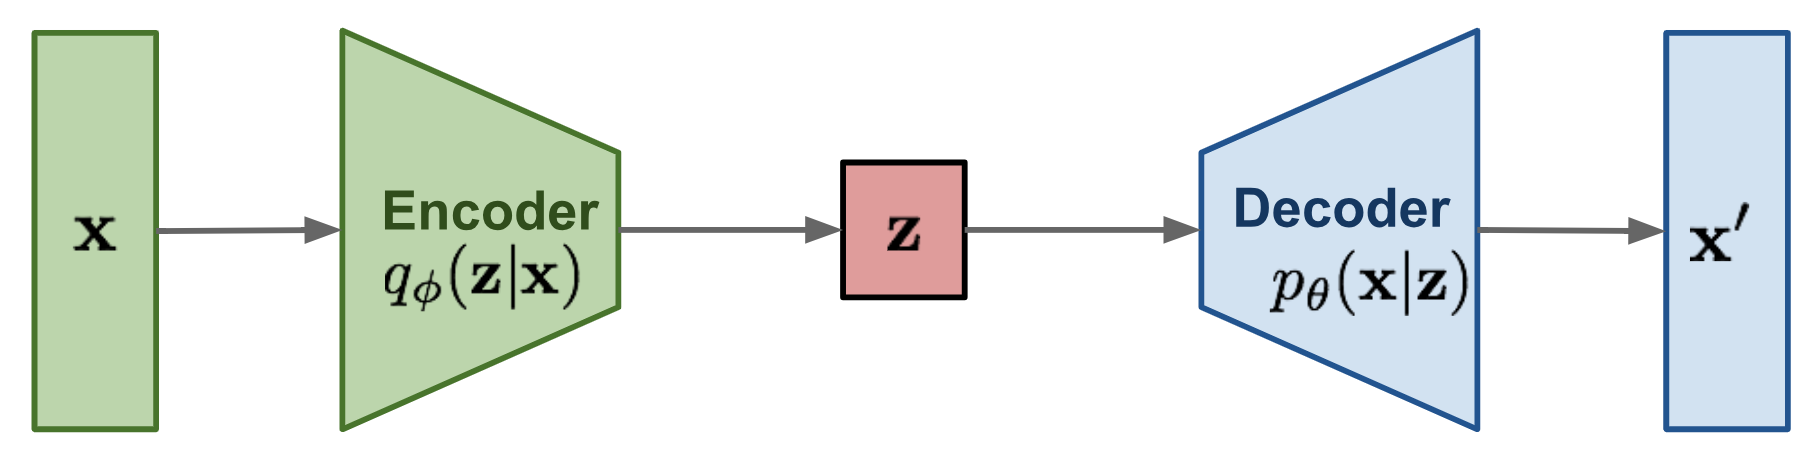
\includegraphics[width=0.8\linewidth]{images/vae.png}
    \end{figure}
\end{frame}
\begin{frame}{Variational Autoencoders (VAEs)}
    \small
    \begin{align*}
        \mathbb{E}_{q_{\phi}(\vz|\vx)}\left[\log{\frac{p(\vx,\vz)}{q_{\phi}(\vz|\vx)}}\right] & = \mathbb{E}_{q_{\phi}(\vz|\vx)}\left[\log{\frac{p_{\theta}(\vx|\vz)p(\vz)}{q_{\phi}(\vz|\vx)}}\right]                                                                                                                                    \\
        \uncover<2->{                                                                         & =\mathbb{E}_{q_{\phi}(\vz|\vx)}\left[\log p_{\theta}(\vx|\vz)\right]+\mathbb{E}_{q_{\phi}(\vz|\vx)}\left[\log\frac{p(\vz)}{q_{\phi}(\vz|\vx)}\right] \\}
        \uncover<3->{                                                                         & =\underbrace{\mathbb{E}_{q_{\phi}(\vz|\vx)}\left[\log p_{\theta}(\vx|\vz)\right]}_{\textrm{reconstruction term}}+\underbrace{D_{\mathrm{KL}}(q_{\phi}(\vz|\vx)\parallel p(\vz))}_{\textrm{prior matching term}} \\}
    \end{align*}
    \uncover<3->{
        \normalfont
        \begin{exampleblock}{KL Divergence}
            $D_{\mathrm{KL}}(P\mid\mid Q)=\int p(\vx)\,\log\bigl(\frac{p(\vx)}{q(\vx)}\bigr)\,\mathrm{d}\vx=\mathbb{E}_{P}\left[\log\frac{P(\vx)}{Q(\vx)}\right]$
        \end{exampleblock}
    }
\end{frame}
\begin{frame}{Variational Autoencoders (VAEs)}
    \begin{figure}
        \centering
        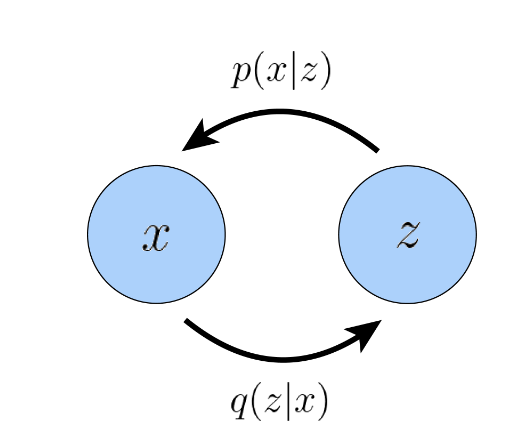
\includegraphics[width=0.5\linewidth]{images/vae_graph.png}
    \end{figure}
\end{frame}
\begin{frame}{Hierarchical Variational Autoencoders (HVAEs)}
    \begin{figure}
        \centering
        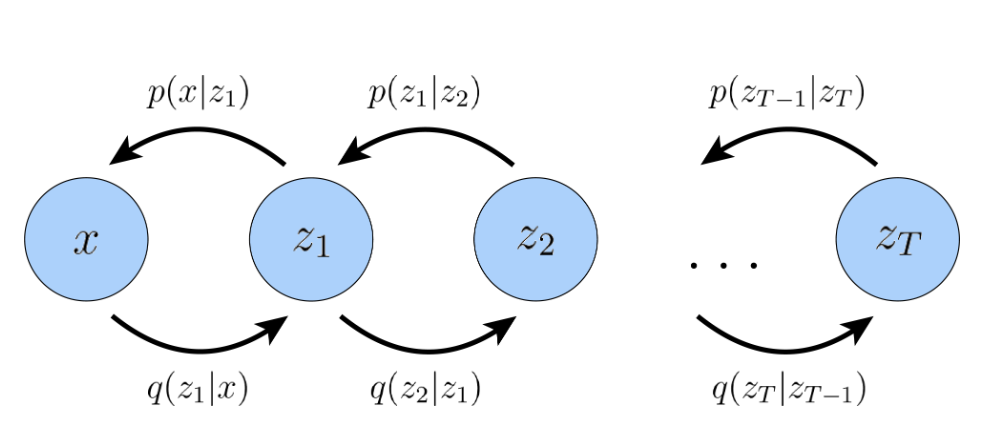
\includegraphics[width=0.9\linewidth]{images/hvae_graph.png}
    \end{figure}
\end{frame}
\begin{frame}{Hierarchical Variational Autoencoders (HVAEs)}

    \small

    \begin{textblock}{8}(0.7, 4.0)
        \begin{itemize}
            \visible<1->{\item In Markovian HVAEs each latent $\vz_{t}$ only conditions on the previous latent $\vz_{t-1}$}
        \end{itemize}
    \end{textblock}

    \begin{textblock}{14}(0.7, 7.0)
        \begin{itemize}
            \visible<2->{\item $\displaystyle p(\vx,\vz_{1:T})=p(\vz_{T})p_{\theta}(\vx|\vz_{1})  \prod^{T}_{t=2}{p_{\theta}(\vz_{t-1}|\vz_{t})}$}
                  \visible<2->{\item $\displaystyle q_{\phi}(\vz_{1:T}|\vx)=q_{\phi}(\vz_{1}|\vx)\prod_{t=2}^{T}q_{\phi}(\vz_{t}|\vz_{t-1})$}
                  \visible<3->{\item $\displaystyle \log p(\vx) \geq \mathbb{E}_{q_{\phi}(\vz_{1:T}|\vx)}\left[\log{\frac{p(\vz_{T})p_{\theta}(\vx|\vz_{1})\prod_{t=2}^{T}p_{\theta}(\vz_{t-1}|\vz_{t})}{q_{\phi}(\vz_{1}|\vx)\prod_{t=2}^{T}q_{\phi}(\vz_{t}|\vz_{t-1})}}\right]$}
        \end{itemize}
    \end{textblock}

    \begin{textblock}{6}(9.0, 3.5)
        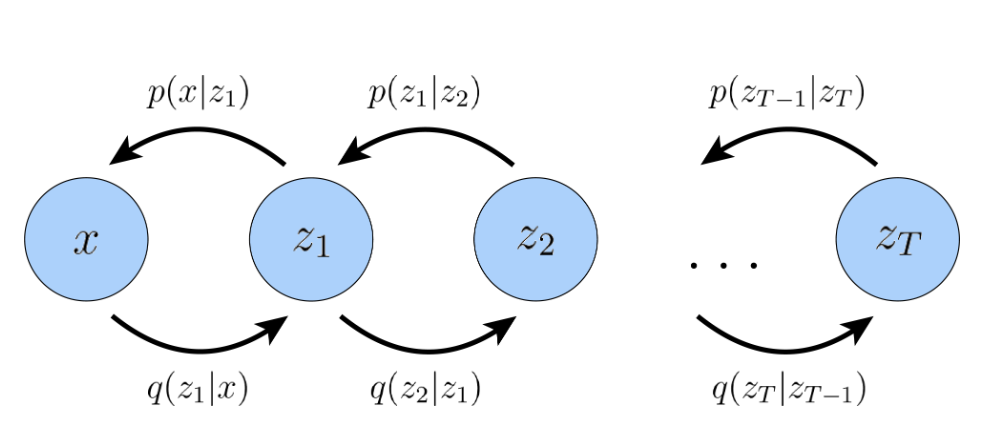
\includegraphics[width=1.0 \textwidth]{images/hvae_graph.png}
    \end{textblock}
\end{frame}
\begin{frame}{Variational Diffusion Models (VDMs)}
    \begin{figure}
        \begin{itemize}
            \setlength{\itemsep}{8pt}
            \item a VDM is a Markovian HVAE with three restrictions:
                  \begin{itemize}
                      \setlength{\itemsep}{8pt}
                      \visible<2->{\item $\vx, \vz \in \mathbb{R}^{D}$}
                            \visible<3->{\item $ \displaystyle q(\vx_{t}|\vx_{t-1})={\mathcal{N}}(\vx_{t};{\sqrt{\alpha_{t}}}\vx_{t-1},(1-\alpha_{t}){\mathbf{I}})$}
                            \visible<4->{\item $ \displaystyle p(\vx_{T})=\mathcal{N}(\vx_{T};0,\mathbf{I})$}
                  \end{itemize}
        \end{itemize}
    \end{figure}
\end{frame}
\begin{frame}{Variational Diffusion Models (VDMs)}
    \begin{figure}
        \centering
        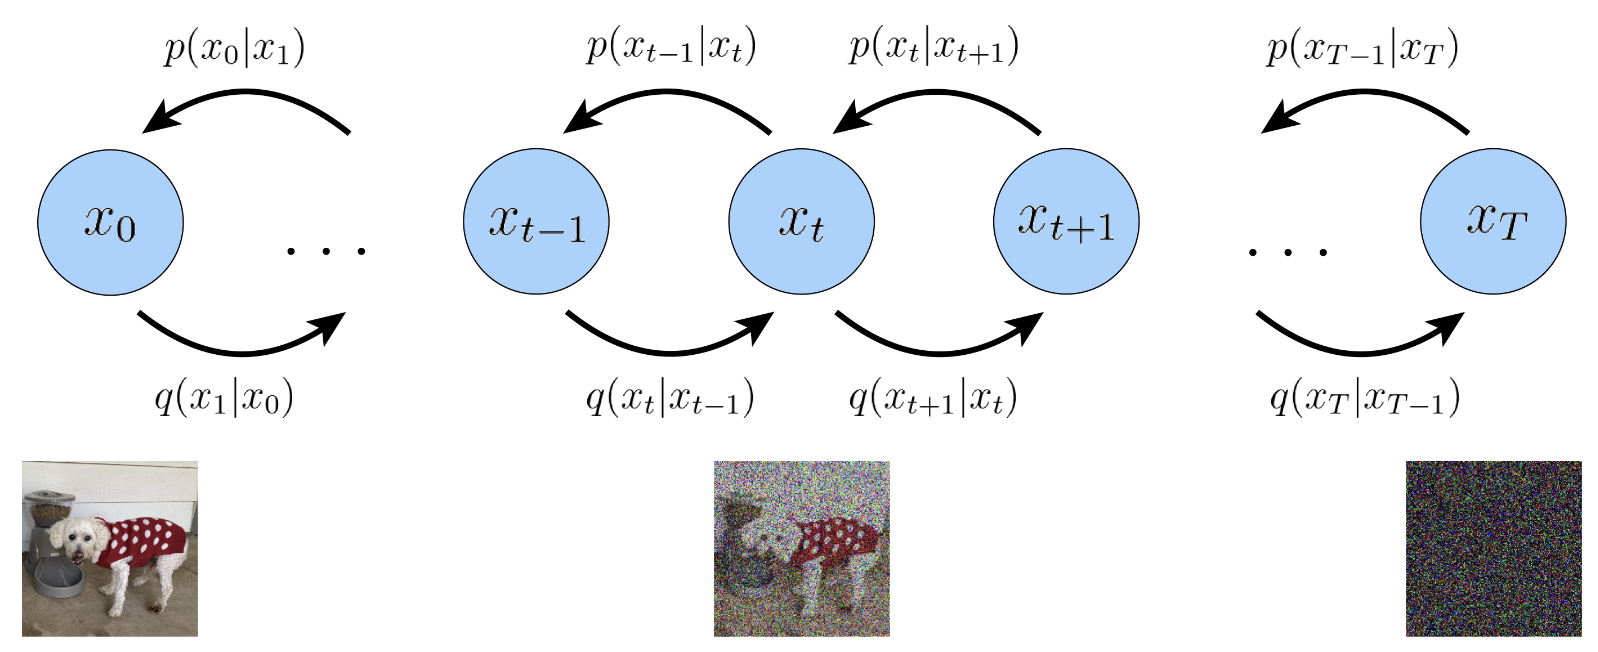
\includegraphics[width=0.9\linewidth]{images/vdm_process.png}
    \end{figure}
\end{frame}
\begin{frame}{Variational Diffusion Models (VDMs)}
    \begin{figure}
        \begin{itemize}
            \setlength{\itemsep}{8pt}
            \item a VDM is a Markovian HVAE with three restrictions:
                  \begin{itemize}
                      \setlength{\itemsep}{8pt}
                      \visible<1->{\item $\vx, \vz \in \mathbb{R}^{D}$}
                            \visible<1->{\item $ \displaystyle q(\vx_{t}|\vx_{t-1})={\mathcal{N}}(\vx_{t};{\sqrt{\alpha_{t}}}\vx_{t-1},(1-\alpha_{t}){\mathbf{I}})$}
                            \visible<1->{\item $ \displaystyle p(\vx_{T})=\mathcal{N}(\vx_{T};0,\mathbf{I})$}
                  \end{itemize}
                  \visible<2->{\item $ \displaystyle \log p(\vx) = \log\int p(\vx_{0:T})d \vx_{1:T}$}
        \end{itemize}
    \end{figure}
\end{frame}
\begin{frame}{Is that the VDM ELBO in your pocket or are you just pleased to see me?}
    \vspace{-1.4em}
    \begin{align*}
        \log p(\vx) = & \log\int p(\vx_{0:T})d \vx_{1:T}                                                                                                                                                                \\
        \ge           & \underbrace{\mathbb{E}_{q(\vx_{1}|\vx_{0})}\left[\log p_{\theta}(\vx_{0}|\vx_{1})\right]}_{\textrm{reconstruction term}}                                                                        \\
                      & - \underbrace{\mathbb{E}_{q(\vx_{T-1}|\vx_{0})}\left[D_{\mathrm{KL}}(q(\vx_{T}|\vx_{T-1}) \parallel p(\vx_{T}))\right]}_{\textrm{prior matching term}}                                          \\
                      & -\sum_{t=1}^{T-1}\underbrace{\mathbb{E}_{q(\vx_{t-1},\vx_{t+1}|\vx_{0})}\left[D_{\mathrm{KL}}(q(\vx_{t}|\vx_{t-1}) \parallel p_{\theta}(\vx_{t}|\vx_{t+1}))\right]}_{\textrm{consistency term}} \\
    \end{align*}
\end{frame}
\begin{frame}{Variational Diffusion Models (VDMs)}
    \begin{figure}
        \centering
        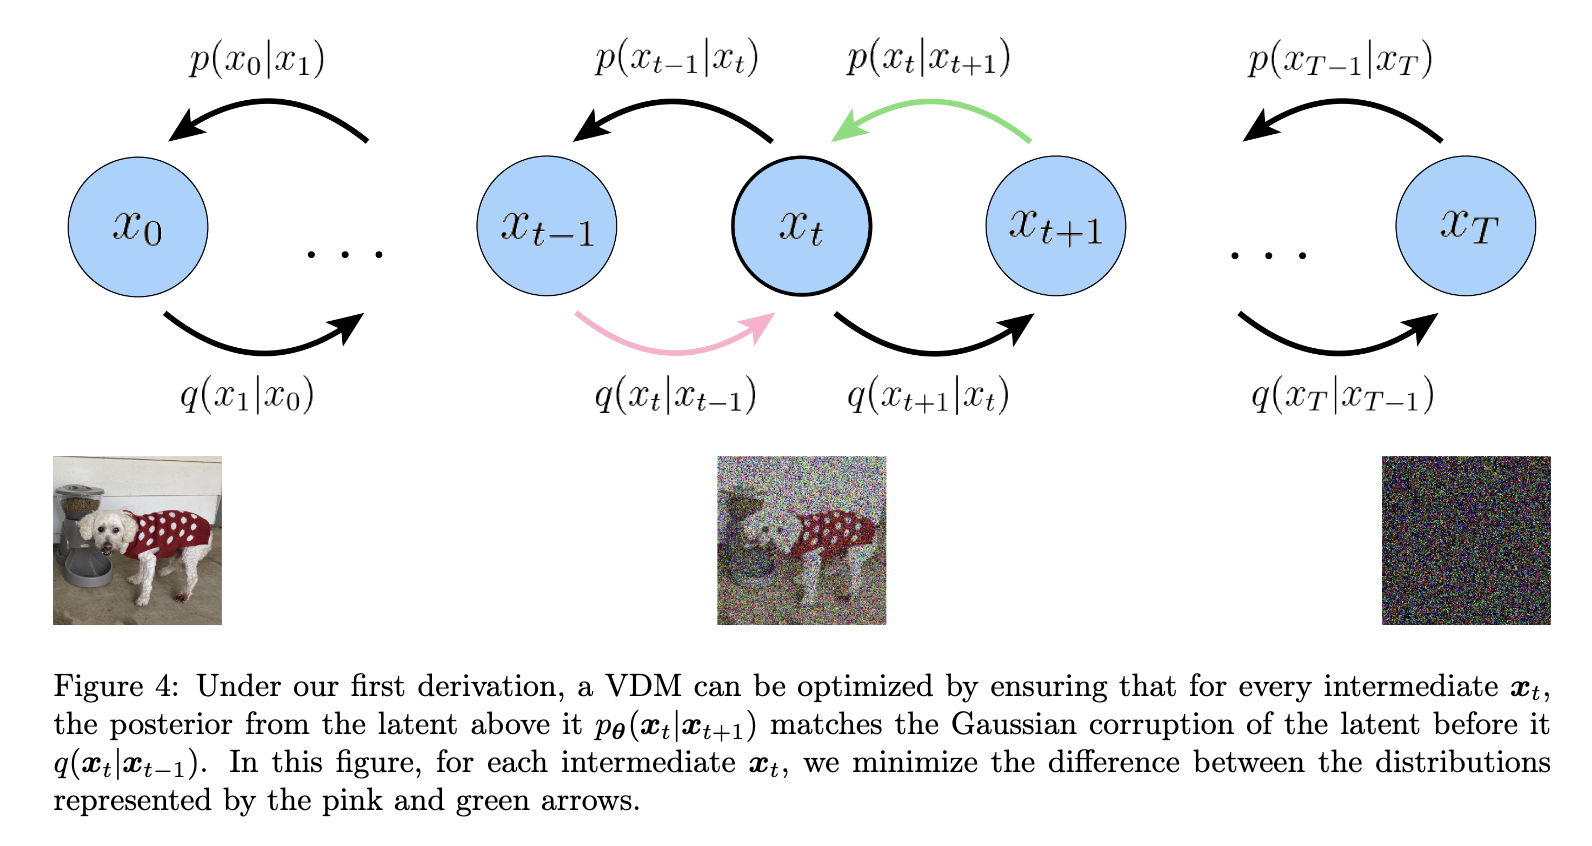
\includegraphics[width=0.9\linewidth]{images/vdm_fig4.png}
    \end{figure}
\end{frame}
\begin{frame}{Lower variance estimator of the VDM ELBO}
    \vspace{0em}
    \setlength{\jot}{10pt}
    \begin{align*}
        \visible<1-1>{\log p(\vx) \ge & \ldots -\sum_{t=1}^{T-1}\underbrace{\mathbb{E}_{q(\vx_{t-1},\vx_{t+1}|\vx_{0})}\left[D_{\mathrm{KL}}(q(\vx_{t}|\vx_{t-1}) \parallel p_{\theta}(\vx_{t}|\vx_{t+1}))\right]}_{\textrm{consistency term}}}                         \\
        \visible<2->{\log p(\vx) \ge  & \underbrace{\mathbb{E}_{q(\vx_{1}|\vx_{0})}\left[\log p_{\theta}(\vx_{0}|\vx_{1})\right]}_{\textrm{reconstruction term}} - \underbrace{D_{\mathrm{KL}}(q(\vx_{T}|\vx_{0}) \parallel p(\vx_{T}))}_{\textrm{prior matching term}} \\
                                      & -\sum_{t=2}^{T}\underbrace{\mathbb{E}_{q(\vx_{t}|\vx_{0})}\left[D_{\mathrm{KL}}(q(\vx_{t-1}|\vx_{t},\vx_{0}) \parallel p_{\theta}(\vx_{t-1}|\vx_{t}))\right]}_{\textrm{denoising matching term}}}                               \\
    \end{align*}
\end{frame}
\begin{frame}{Lower variance estimator of the VDM ELBO}
    \begin{figure}
        \centering
        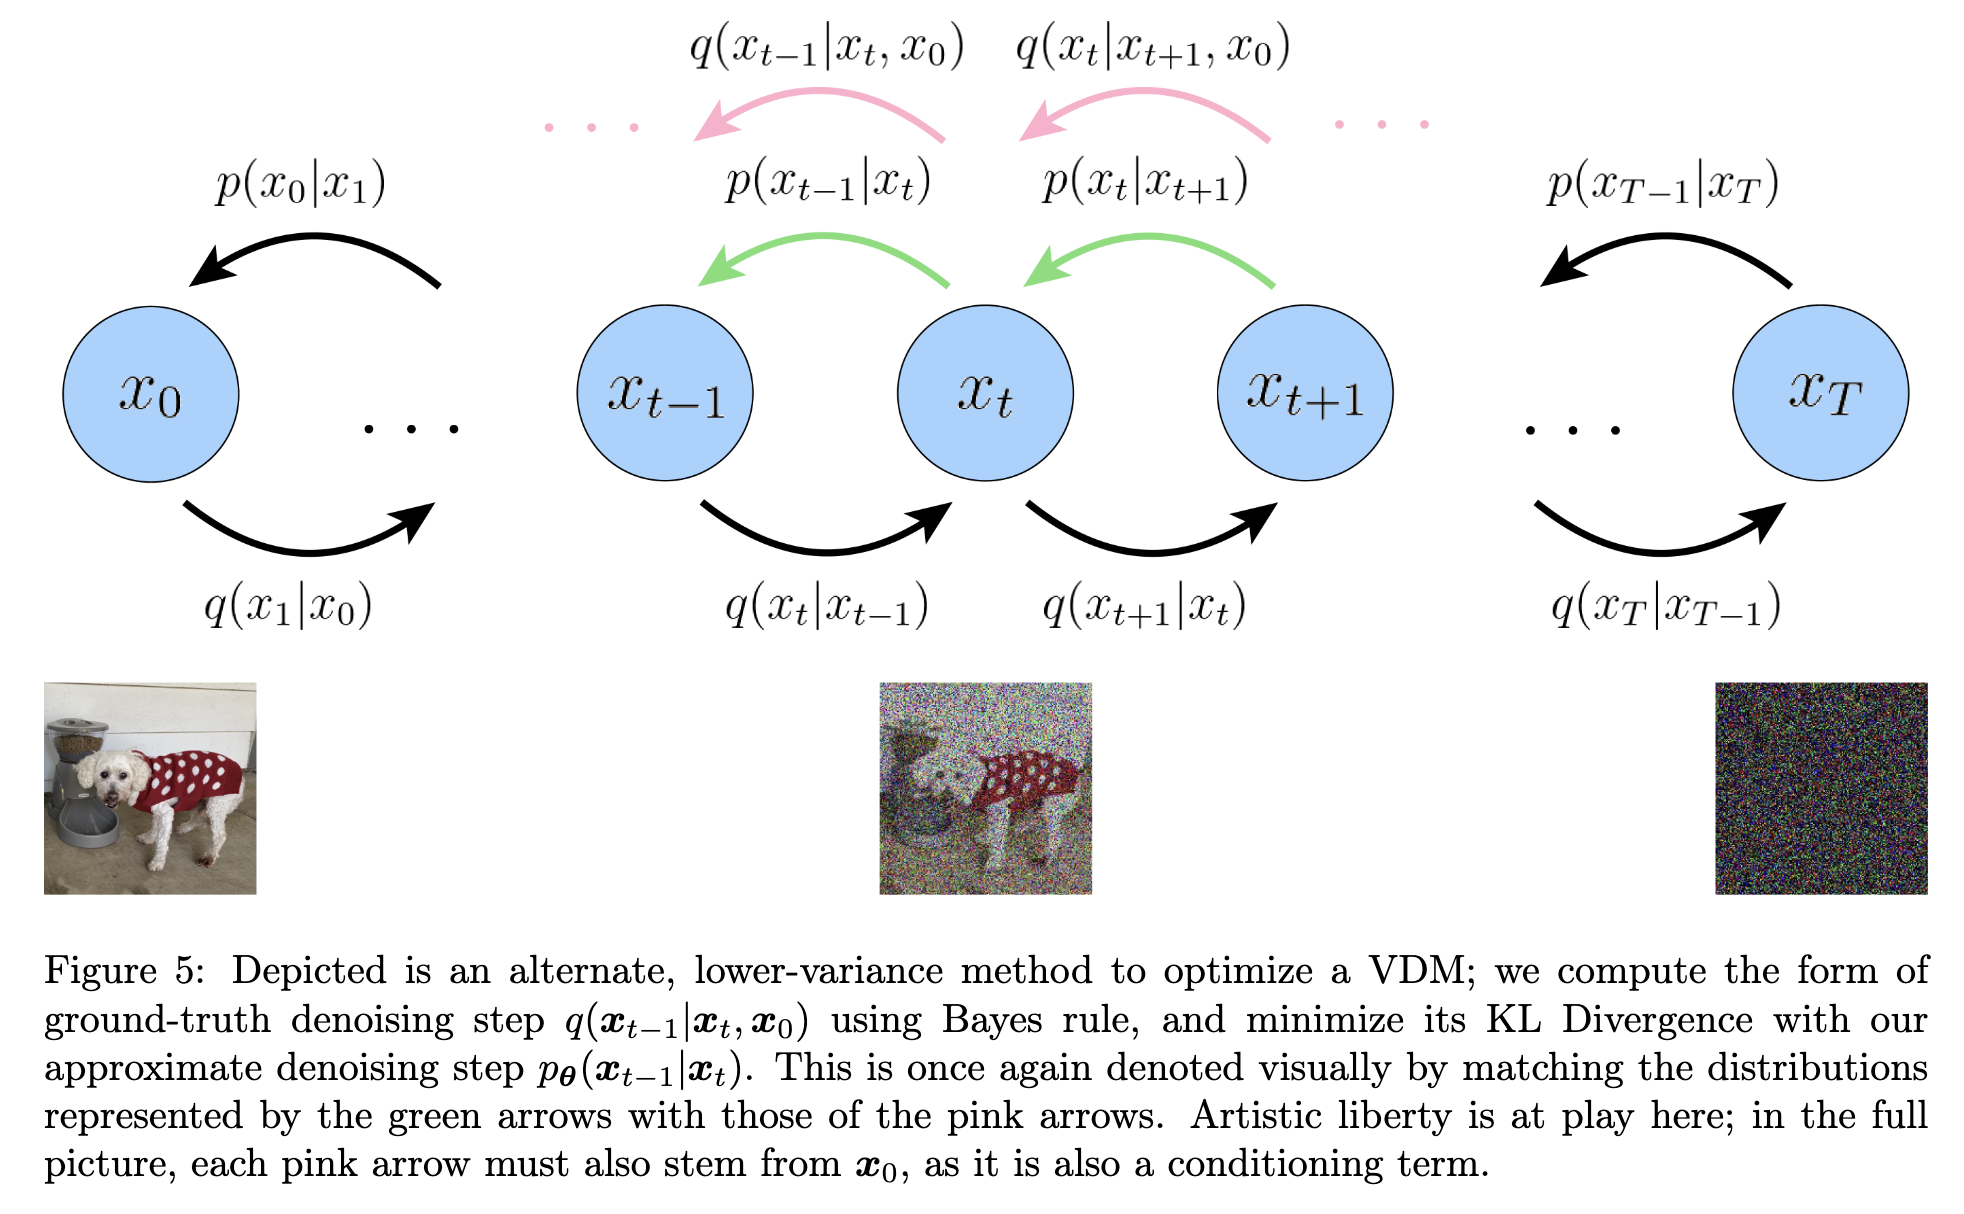
\includegraphics[width=0.8\linewidth]{images/vdm_fig5.png}
    \end{figure}
\end{frame}
\begin{frame}{Ground truth denoiser}
    \vspace{-1em}
    \small
    \setlength{\jot}{10pt}
    \begin{align*}
        \visible<1->{q(\vx_{t-1}|\vx_{t},\vx_{0})}         & \visible<2->{= \frac{q(\vx_{t}|\vx_{t-1},\vx_{0})q(\vx_{t-1}|\vx_{0})}{q(\vx_{t}|\vx_{0})}}                                                                                                                                                                               \\
                                                           & \only<3-4>{= \frac{\mathcal{N}(\vx_{t};\sqrt{\alpha_{t}}\vx_{t-1},(1-\alpha_{t})\mathbf{I})\mathcal{N}(\vx_{t-1};\sqrt{\bar{\alpha}_{t-1}}\vx_{0},(1-\bar{\alpha}_{t-1})\mathbf{I})}{\mathcal{N}(\vx_{t};\sqrt{\bar{\alpha}_{t}}\vx_{0},(1-\bar{\alpha}_{t})\mathbf{I})}} \\
                                                           & \visible<4-5>{= \mathcal{N} (\vx_{t-1};\frac{\sqrt{\alpha_{t}}(1-\bar{\alpha}_{t-1})\vx_{t}+\sqrt{\bar{\alpha}_{t-1}}(1-\alpha_{t})\vx_{0}}{1-\bar{\alpha}_{t}},\frac{(1-\alpha_{t})(1-\bar{\alpha}_{t-1})}{1-\bar{\alpha}_{t}}\mathbf{I})}                               \\
                                                           & \visible<5->{= \mathcal{N}(\vx_{t-1};\boldsymbol{\mu}_{q}(\vx_{t},\vx_{0}),\boldsymbol{\Sigma}_{q}(t))}                                                                                                                                                                   \\
        \visible<6->{\boldsymbol{\mu}_{q}(\vx_{t},\vx_{0}) & = \frac{\sqrt{\alpha_{t}}(1-\bar{\alpha}_{t-1})\vx_{t}+\sqrt{\bar{\alpha}_{t-1}}(1-\alpha_{t})\vx_{0}}{1-\bar{\alpha}_{t}}}                                                                                                                                               \\
        \visible<6->{\boldsymbol{\Sigma}_{q}(t)            & = \sigma^{2}_{q}(t)\mathbf{I}, \quad \sigma^{2}_{q}(t) = \frac{(1-\alpha_{t})(1-\bar{\alpha}_{t-1})}{1-\bar{\alpha}_{t}}}
    \end{align*}
\end{frame}
\begin{frame}{Parameterised denoiser}
    % \begin{columns}
    %     \begin{column}{0.5\textwidth}
    \vspace{0em}
    \small
    \begin{itemize}
        \setlength\itemsep{1em}
        \visible<1->{\item We want to learn $\ \displaystyle p_{\boldsymbol{\theta}}(\vx_{t-1}|\vx_{t}) \approx \mathcal{N}(\vx_{t-1};\boldsymbol{\mu}_{q}(\vx_{t},\vx_{0}),\boldsymbol{\Sigma}_{q}(t))$}
              \visible<2->{\item $\displaystyle \boldsymbol{\Sigma}_{q}(t) = \sigma^{2}_{q}(t)\mathbf{I}\ $ is known}
              \visible<3->{\item We parameterise $\displaystyle \boldsymbol{\mu}_{\boldsymbol{\theta}}(\vx_{t}, t)$ as $\displaystyle p_{\boldsymbol{\theta}}(\vx_{t-1}|\vx_{t})$ does not condition on $\displaystyle \vx_{0}$}
              \visible<4->{\item
              $ \displaystyle
                  \!
                  \begin{aligned}[t]
                        & \ \underset{\boldsymbol{\theta}}{\argmin}\ D_{\mathrm{KL}}(q(\vx_{t-1}|\vx_{t},\vx_{0})\parallel  p_{\boldsymbol{\theta}}(\vx_{t-1}|\vx_{t}))              \\
                      = & \ \underset{\boldsymbol{\theta}}{\argmin}\ {\frac{1}{2\sigma_{q}^{2}(t)}}\Big[\|\boldsymbol{\mu}_{\boldsymbol{\theta}}-\boldsymbol{\mu}_{q}\|_{2}^{2}\Big]
                  \end{aligned}
              $}

    \end{itemize}
    %     \end{column}
    % \end{columns}


\end{frame}

\usebeamertemplate{endpage}

\begin{frame}{Rewriting the encoder step $\vx_{t} \sim q(\vx_{t}|\vx_0)$}
  \begin{figure}
    \centering
    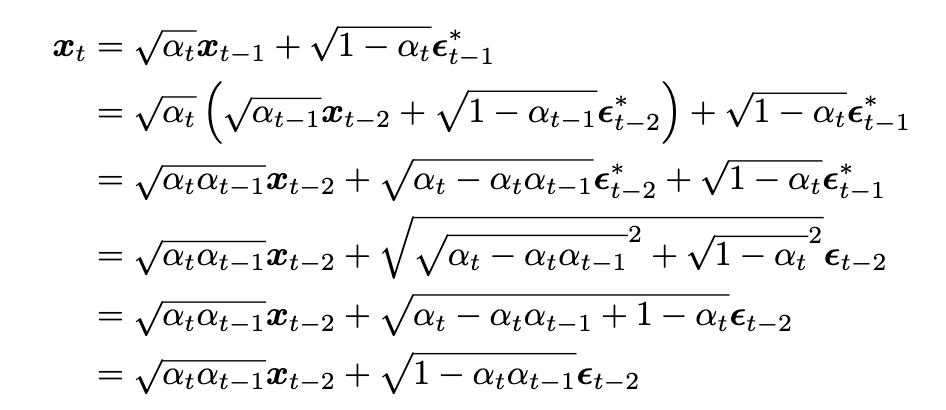
\includegraphics[width=0.8\linewidth]{images/encoder_step1.png}
  \end{figure}
\end{frame}
\begin{frame}{Rewriting the encoder step $\vx_{t} \sim q(\vx_{t}|\vx_0)$}
  \begin{figure}
    \centering
    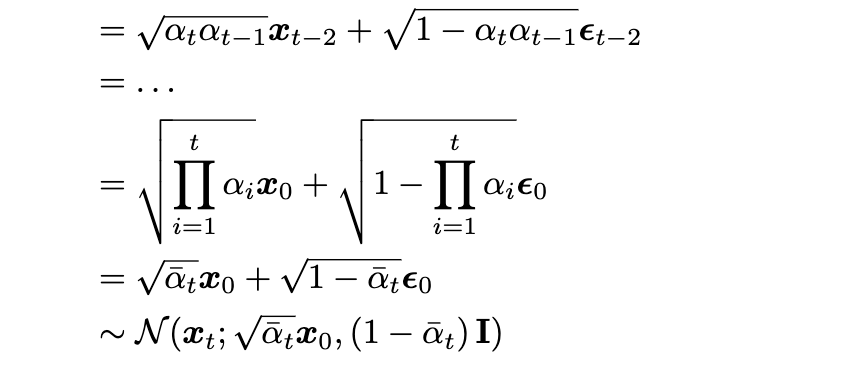
\includegraphics[width=0.8\linewidth]{images/encoder_step2.png}
  \end{figure}
\end{frame}

\end{document}